\documentclass[crop,border=0pt]{standalone}

\usepackage{mathtools}
\usepackage{tikz}
\usetikzlibrary{positioning,scopes,arrows}

\begin{document}
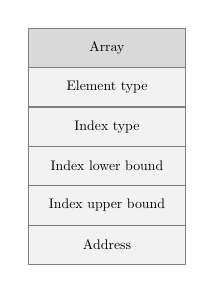
\begin{tikzpicture}[scale=0.5, every node/.style={scale=0.5,black}]
  {[xstep=4cm, ystep=1cm, gray, thin]

    \draw[fill=gray!10] (0,0) grid (4, 5) rectangle (0,0);
    \draw[fill=gray!30] (0,5) grid (4, 6) rectangle (0,5);

    \node at (2, 5.5) {Array};
    \node at (2, 4.5) {Element type};
    \node at (2, 3.5) {Index type};
    \node at (2, 2.5) {Index lower bound};
    \node at (2, 1.5) {Index upper bound};
    \node at (2, 0.5) {Address};
  }

\end{tikzpicture}
\end{document}
